\documentclass[tikz,border=5mm,12pt]{standalone}

\def\vsep{12.5mm}

\begin{document}
  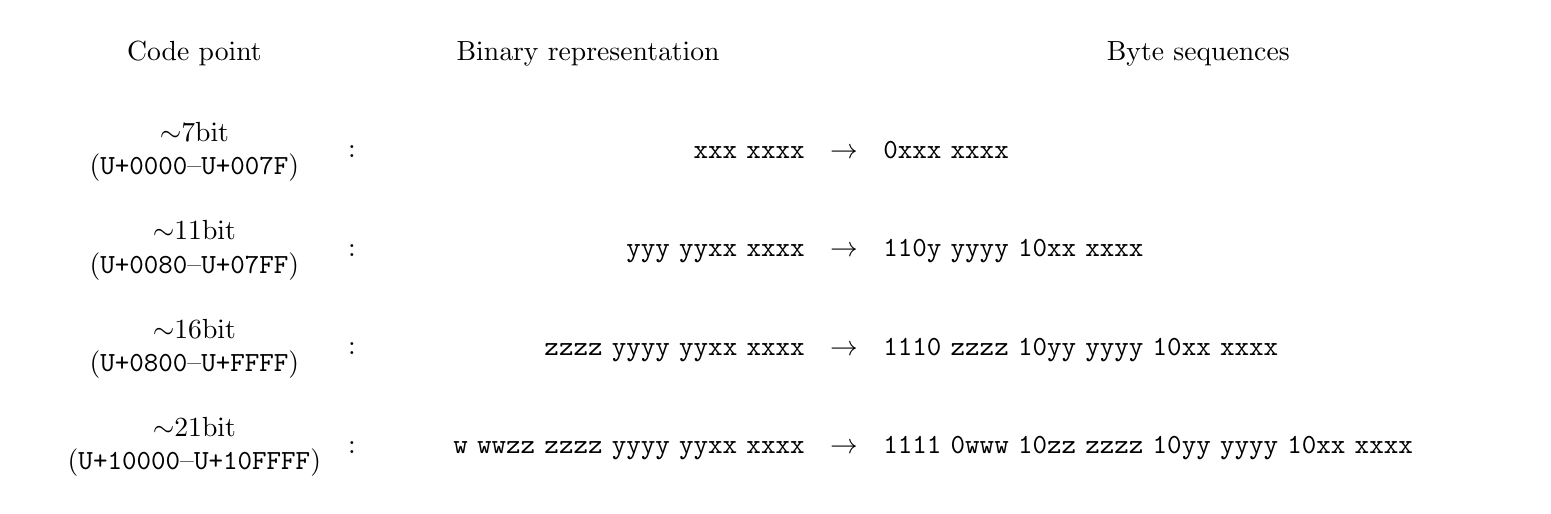
\begin{tikzpicture}
    \node[text width=40mm,align=center] at (0,0) {Code point\strut};
    \node[text centered,text width=40mm] at (0,-1*\vsep) {
      $\sim$7bit \\
      (\texttt{U+0000}--\texttt{U+007F})};
    \node[text centered,text width=40mm] at (0,-2*\vsep) {
      $\sim$11bit \\
      (\texttt{U+0080}--\texttt{U+07FF})};
    \node[text centered,text width=40mm] at (0,-3*\vsep) {
      $\sim$16bit \\
      (\texttt{U+0800}--\texttt{U+FFFF})};
    \node[text centered,text width=40mm] at (0,-4*\vsep) {
      $\sim$21bit \\
      (\texttt{U+10000}--\texttt{U+10FFFF})};

    \node at (20mm,-1*\vsep) {:};
    \node at (20mm,-2*\vsep) {:};
    \node at (20mm,-3*\vsep) {:};
    \node at (20mm,-4*\vsep) {:};

    \node[text width=55mm,align=center] at (50mm,0) {Binary representation\strut};
    \node[align=right,text width=55mm] at (50mm,-1*\vsep) {\texttt{xxx xxxx}\strut};
    \node[align=right,text width=55mm] at (50mm,-2*\vsep) {\texttt{yyy yyxx xxxx}\strut};
    \node[align=right,text width=55mm] at (50mm,-3*\vsep) {\texttt{zzzz yyyy yyxx xxxx}\strut};
    \node[align=right,text width=55mm] at (50mm,-4*\vsep) {\texttt{w wwzz zzzz yyyy yyxx xxxx}\strut};

    \node at (82.5mm,-1*\vsep) {$\rightarrow$\strut};
    \node at (82.5mm,-2*\vsep) {$\rightarrow$\strut};
    \node at (82.5mm,-3*\vsep) {$\rightarrow$\strut};
    \node at (82.5mm,-4*\vsep) {$\rightarrow$\strut};

    \node[text width=80mm,align=center] at (127.5mm,0) {Byte sequences};
    \node[align=left,text width=80mm] at (127.5mm,-1*\vsep) {\texttt{0xxx xxxx}\strut};
    \node[align=left,text width=80mm] at (127.5mm,-2*\vsep) {\texttt{110y yyyy 10xx xxxx}\strut};
    \node[align=left,text width=80mm] at (127.5mm,-3*\vsep) {\texttt{1110 zzzz 10yy yyyy 10xx xxxx}\strut};
    \node[align=left,text width=80mm] at (127.5mm,-4*\vsep) {\texttt{1111 0www 10zz zzzz 10yy yyyy 10xx xxxx}\strut};

  \end{tikzpicture}
\end{document}
